\chapter{The Search for the Supersymmetric Top-quark}
\label{chap:search_stop}

\epigraph{
\textit{It will be remembered that the 18$^{th}$ century was, on the whole,
addicted to an ascending series of living forms shading by insensible degrees
into each other and leading onto man.
There was no consideration of the fact that this might be reading into Nature a greater
unity than she actually possessed. It led inevitibly to some highly
questionable taxonomy produced in the effort to compress all life into positions upon a
single stairway.}
}
{
--Loren Eiseley, \textit{Darwin's Century}
}

\epigraph{
\textit{Cease, cows, life is short.}
}
{
--Gabriel Garc\'{i}a M\'{a}rquez, \textit{One Hundred Years of Solitude}
}

%%%%%%%%%%%%%%%%%%%%%%%%%%%%%%%%%%%%%%%%%%%%%%%%%%%%%%%%%%%%%%%%%%%%%%%%%%%%%%%%%%%%%%%%
%%%%%%%%%%%%%%%%%%%%%%%%%%%%%%%%%%%%%%%%%%%%%%%%%%%%%%%%%%%%%%%%%%%%%%%%%%%%%%%%%%%%%%%%
%%%%%%%%%%%%%%%%%%%%%%%%%%%%%%%%%%%%%%%%%%%%%%%%%%%%%%%%%%%%%%%%%%%%%%%%%%%%%%%%%%%%%%%%
%%%%%%%%%%%%%%%%%%%%%%%%%%%%%%%%%%%%%%%%%%%%%%%%%%%%%%%%%%%%%%%%%%%%%%%%%%%%%%%%%%%%%%%%

As described in Chapter~\ref{chap:bsm}, the lighter mass eigenstate of the superpartner of
the top quark, $\stopone$, plays an important role in helping solve the Hierarchy problem.
Most SUSY scenarios prefer \stopone masses not much larger than $1\,\TeV$, so as to keep them
at the scale EWSB.
%particularly if the \stopone mass is not too massive, preferably not much heavier than $1\,\TeV$.
If the \stopone exists, and is indeed lighter than the \TeV scale, it may easily be produced in the $13\,\TeV$ $pp$ collisions
occurring at the LHC.
Searches for stops therefore play a prominent role in the searches for SUSY in ATLAS.

This chapter therefore presents a search for the production of stop quarks.
The SUSY model considered here satisfies $R$-parity conservation, as do the majority of SUSY
searches at the LHC, which forces the \stopone to be produced in pairs and to follow
a decay chain ending in the LSP.
The LSP in these models is assumed to be the lights neutralino, \ninoone.

\begin{figure}[!htb]
    \begin{center}
        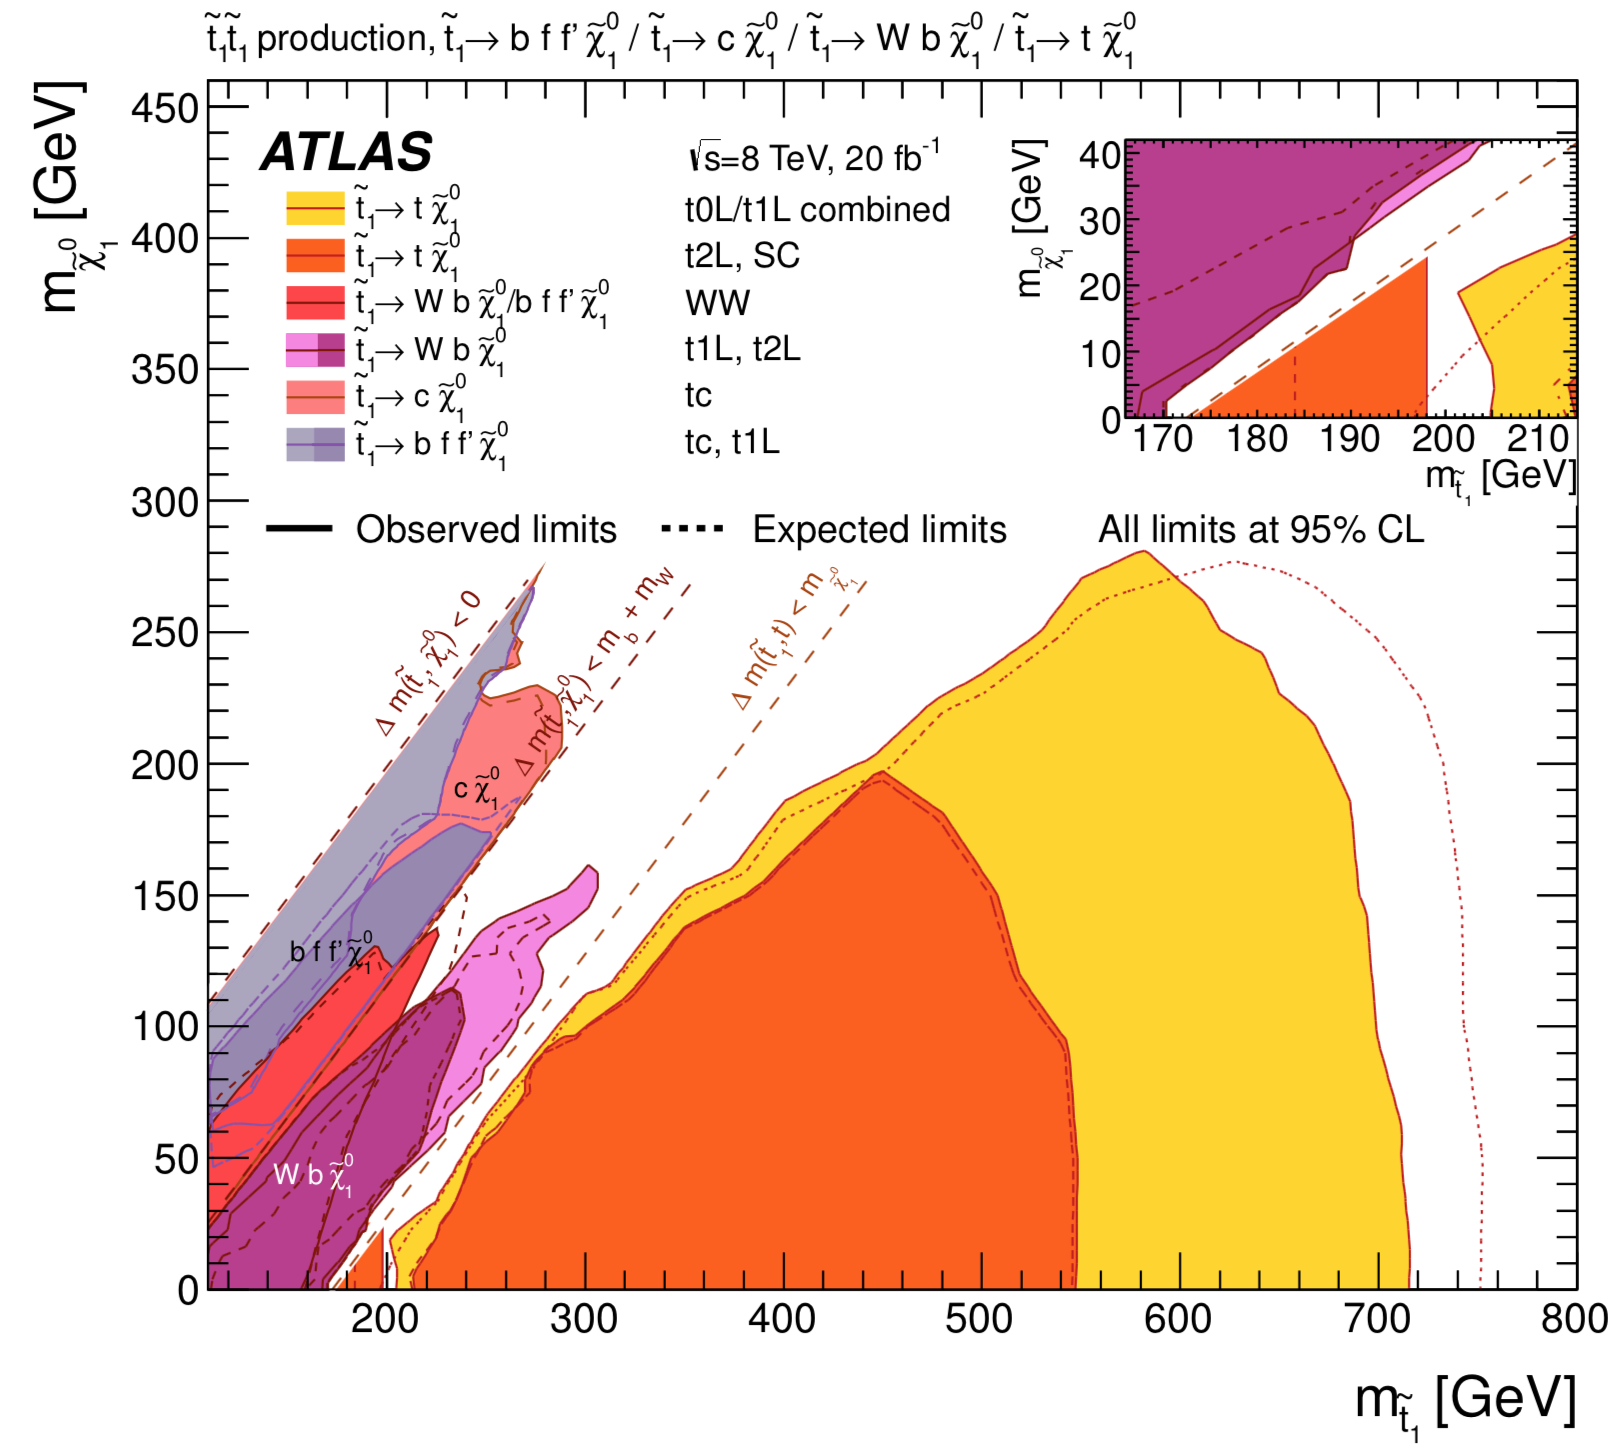
\includegraphics[width=0.7\textwidth]{figures/search_stop2l/run1_stop_summary}
        \caption{
        }
        \label{fig:run1_stop_summary}
    \end{center}
\end{figure}

%\chinoonepm
%
%\ninoone
%
%\ninotwo
%
%\stopone
%
%\stoptwo
%
%\stopL
%
%\stopR
%
%\slepton
%
%\sleptonL
%
%\sleptonR
